\section{Work and Energy}

Energy gives us one more tool to use to analyze physical situations.
When forces and accelerations are used, you usually freeze the action at
a particular instant in time, draw a free-body diagram, set up force
equations, figure out accelerations, etc.  With energy the approach is
usually a little different.  Often you can look at the starting
conditions (initial speed and height, for instance) and the final
conditions (final speed and height), and not have to worry about what
happens in between.  The initial and final information can often tell
you all you need to know.

\subsection{Work}

Energy is defined as the ability to do work, but what is work?  In
physics the technical definition of work is the force-displacement path
integral
\begin{equation}
    W=\int_\ini^\fin F_s \dif s
\end{equation}
where
$
    F_s
$ is the component of
$
    \vec{F}
$ in the direction of motion.

We will explain work intuitively through examples.
\begin{remark}
    Work is done whenever a force causes displacement.
\end{remark}
If a system as a whole exerts a force on its surroundings and a
displacement occurs, the work done is called \textbf{external work}.  A
physics teacher pushing papers across his desk is doing external work.
A physics teacher standing motionless is not doing any significant
external work.

If a part of a system exerts a force on another part of the same system
and a displacement occurs, the work done is called \textbf{internal work}.
A physics teacher standing still is doing internal work.  In mechanics,
when we say work has been done we are often referring to external work.

For any system, work is done whenever a force results in a displacement.
Consider the examples below.
\begin{figure}[ht]
    \centering
    \begin{subfigure}{.20\textwidth}
        \centering
        \incfig{textbook-at-rest}
        \caption{No work is done on a textbook when it is held at rest.}
        \label{fig:textbook-at-rest}
    \end{subfigure}
    \hfill
    \begin{subfigure}{.20\textwidth}
        \centering
        \incfig{textbook-pushed-up}
        \caption{Positive work is done on a textbook when it is raised
        vertically at a constant velocity.}%
        \label{fig:textbook-pushed-up}
    \end{subfigure}
    \hfill
    \begin{subfigure}{.20\textwidth}
        \centering
        \incfig{textbook-pushed-diagonally}
        \caption{Positive work is also done on a textbook when it is
        raised diagonally at a constant velocity.}%
        \label{fig:textbook-pushed-diagonally}
    \end{subfigure}
\end{figure}

Figure~%
\ref{fig:textbook-at-rest} makes sense.  Holding a book at rest results
in no work being done.  Figure~%
\ref{fig:textbook-pushed-up} and Figure~%
\ref{fig:textbook-pushed-diagonally} also makes sense.  The teacher
pushes on the book and it moves.  Work was done.

Consider three more examples below.
\begin{figure}[ht]
    \centering
    \begin{subfigure}{.25\textwidth}
        \centering
        \incfig{textbook-pushed-while-moving}
        \caption{No work is done on a textbook when it is carried
        horizontally at a constant velocity.}%
        \label{fig:textbook-pushed-while-moving}
    \end{subfigure}
    \hfill
    \begin{subfigure}{.25\textwidth}
        \centering
        \incfig{textbook-pushed-while-lowering-diagonally}
        \caption{Negative work is done on a textbook when it is lowered
        diagonally at a constant velocity.}%
        \label{fig:textbook-pushed-while-lowering-diagonally}
    \end{subfigure}
    \hfill
    \begin{subfigure}{.25\textwidth}
        \centering
        \incfig{textbook-pushed-while-lowering}
        \caption{Negative work is also done on a textbook when it is
        lowered vertically at a constant velocity.}%
        \label{fig:textbook-pushed-while-lowering}
    \end{subfigure}
\end{figure}

Figure~%
\ref{fig:textbook-pushed-while-moving} is counterintuitive.  Work is
done on an object whenever force \emph{causes} a displacement.  In this
example, the force applied is vertical but the displacement is
horizontal.  How does a vertical force affect horizontal motion?  It
doesn't.  Work is done whenever a force, or a \textbf{component} of a
force results in a displacement.

Looking at Figure~%
\ref{fig:textbook-pushed-while-lowering-diagonally} and Figure~%
\ref{fig:textbook-pushed-while-lowering} we see negative work being
done.  When force and the displacement on the object are parallel it
means all the force is displacing the object and doing work.  When force
and is not quite parallel to displacement, it means only a certain
component of the force is affecting the displacement causing less
displacement.  When the angle between the force and displacement reaches
$
    \qty{\frac{1}{2}\pi}{\radian}
$ it means the component of the force parallel to the displacement is
zero meaning now work is being done.  The farther the two vectors get
from parallel, the less work is done.  Expand the angle beyond
$
    \qty{\frac{1}{2}\pi}{\radian}
$%
, force and displacement are pointing in opposite directions.  This is
negative work, when you apply less than no force.

\subsubsection{Constant Force}

Figure~%
\ref{fig:work-constant-force} shows a particle being acted upon by a
constant force
$
    \vec{F}
$ over displacement
$
    \Delta \vec{r}
$%
.  The force component along the direction of motion is
\begin{equation}
    F_s = F\cos{\theta}
\end{equation}
Thus,
\begin{equation}
    W = \int_\ini^\fin F_s \dif s = \int_\ini^\fin F\cos{\theta} \dif s
\end{equation}
Since both
$
    F
$ and
$
    \cos{\theta}
$ are constant over displacement
$
    \Delta r
$%
,
\begin{equation}
    W = F\cos{\theta}\int_\ini^\fin \dif s = F\cos{\theta}(s_\fin - s_\ini)
\end{equation}

\begin{figure}
    \centering
    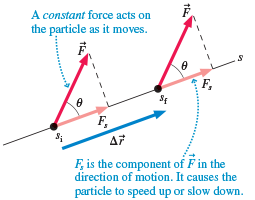
\includegraphics[width=0.4\textwidth]{../figures/work-constant-force.png}
    \caption{Work being done by a constant force}%
    \label{fig:work-constant-force}
\end{figure}

\subsubsection{Variable Force}

To calculate the work done on a object with a changing force, the
definition of work is all you need:
\begin{equation}
    W = \int_\ini^\fin F_s \dif s
\end{equation}
The integral sums up the small amounts of work
$
    F_s
$ and
$
    \dif s
$ done in each step along the trajectory.

\subsection{Energy}

A system possesses \textbf{energy} if it has the ability to do work.
Energy is transferred or transformed whenever work is done.  Energy is\dots
\begin{itemize}
    \item
        a scalar quantity
    \item
        abstract and cannot always be perceived
    \item
        given meaning through calculation
\end{itemize}

Energy can exist in many different forms.  All forms of energy are
either kinetic or potential.  The energy assosciated with motion is
called \textbf{kinetic energy}.  The energy assosciated with position is
called \textbf{potential energy}.

The unit of all forms of energy is the joule:
\begin{equation}
    \left[\unit{\joule} = \unit{\newton\metre} = \unit{\kilo\gram\square\metre\per\square\second}\right]
\end{equation}

\subsubsection{The Energy Principle}

The most important step in energy analysis is to clearly define the
system because we are referring to the energy of something; the energy
of a system.

\begin{figure}
    \centering
    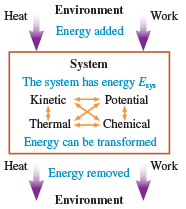
\includegraphics[width=0.4\textwidth]{../figures/system-environment-energy.png}
    \caption{A system-environment perspective on energy.}%
    \label{fig:system-environment-energy}

\end{figure}

Figure~%
\ref{fig:system-environment-energy} shows a system with energy.  Within
the system, energy can be \emph{transformed without loss}.  As long as
the system is not interacting with the environment, the total energy of
the system is unchanged.

Systems do often interact with their environment.  These interactions
changes the energy of the system by increasing it or decreasing it.
There are only two ways to transfer energy.
\begin{itemize}
    \item
        By pushing or pulling through \textbf{work}.
    \item
        By thermal means through \textbf{heat}.
\end{itemize}

The key ideas are \textbf{energy transformation} within a system, and
\textbf{energy transfer} between the system and the environment.

Transformations of energy don't change the total energy within the
system.  \emph{Change} occurs only when there's a transfer of energy
between the system and the environment.  If we treat incoming energy as
a positive transfer and outgoing energy as a negative transfer, and with
work being the only energy transfer process that we consider for now, we
can write
\begin{equation}
    \Delta E_\sys = W_\ext
\end{equation}
where
$
    E_\sys
$ is the energy in the system and
$
    W_\ext
$ is the work done by the environment.  We are saying the net change of
energy in a system is equal to the net work done.  This is referred to
as the \textbf{energy principle}.

\subsubsection{Work and Kinetic Energy}

From Newton's second law, it can be shown that work on a free rigid body
is
\begin{equation}
    W = \Delta K
\end{equation}
where
$
    K = \frac{1}{2}mv^2
$%
.
\begin{proof}
    We model a free rigid body that is acted by one constant force
    $
        \vec{F}
    $ that acts parallel to the direction of motion over displacement
    $
        \Delta s
    $%
    .
    \begin{equation}
        F_s=ma_s=m\od{v_s}{t}
    \end{equation}
    where
    $
        F_s
    $ is the magnitude of force.  With the chain rule, we see how
    velocity changes with postion as opposed to time
    \begin{equation}
        \od{v_s}{t}=\od{s}{t}=v_s\od{v_s}{s}
    \end{equation}
    where
    $
        \od{s}{t} = v_s
    $%
.    Thus, we rewrite Newton's second law as
    \begin{align}
        F_s &= mv_s\od{v_s}{s} \\
        mv_s \dif v_s = F_s \dif s
    \end{align}
    Integrating both sides,
    \begin{equation}
        \int_{v_{\ini s}}^{v_{\fin s}} mv_s \dif v_s = \int_{s_\ini}^{s_\fin}
        F_s \dif s
    \end{equation}
    By the definition of work,
    $
        W=\int F \dif s
    $
    \begin{equation}
        \int_{v_{\ini s}}^{v_{\fin s}} mv_s \dif v_s = W
    \end{equation}
    Solving for the LHS
    \begin{align}
        \int_{v_{\ini s}}^{v_{\fin s}} mv_s \dif v_s &= m \int_{v_{\ini
        s}}^{v_{\fin s}} v_s \dif v_s \\
        &= m\left[\frac{1}{2} v_s^2\right]_{v_{\ini s}}^{v_{\fin s}} \\
        &=\Delta\left(\frac{1}{2} mv^2 \right)
    \end{align}
    where we define
    $
        K=\frac{1}{2}mv^2
    $%
.    Thus,
    \begin{equation}
        W = \Delta K
    \end{equation}
    $
        \blacksquare
    $
\end{proof}
We define
$
    K
$ as \textbf{kinetic energy}.  Thus, for a free rigid body, work is
equal to the change of kinetic energy.

\subsubsection{Potential Energy}

\begin{figure}
    \centering
    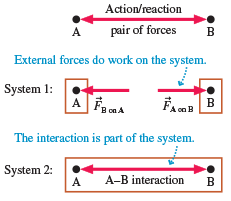
\includegraphics[width=0.4\textwidth]{../figures/two-choices-of-systems.png}
    \caption{Two choices of systems and environment.}%
    \label{fig:two-choies-of-systems}
\end{figure}

Figure~%
\ref{fig:two-choies-of-systems} shows two particles
$
    A
$ and
$
    B
$ that interact with eachother.  There are two ways to define the
system:  system 1 only comsists of the particles; the forces are
external.  By the energy principle, for system 1
\begin{align}
    \Delta E_{\sys 1} &= \Delta K_\tot \\
    &= \Delta W_\ext = W_A + W_B \\
    &= \left[\int \arpair{B}{A} \dif s\right] + \left[\int \arpair{A}{B}
    + \dif s\right]
\end{align}
where the work of the two forces changes the system's kinetic energy.

Now consider system 2, where the interaction is \textbf{internal} to the
system.  Thus,
$
    W_\ext = 0
$%
.  Consequently, the energy principle for system 2 is
\begin{equation}
    \Delta E_{\sys 2} = W_\ext = 0
\end{equation}
from system 1, we know that the kinetic energy changes over displacement
$
    \Delta s
$ so how can
$
    \Delta E_{\sys 2} = 0
$%
?

Because system 2 has an interaction inside that system 1 lacks, we
postulate system 2 has an additional form of energy assosciated with the
interaction.  That is, system 1 has
$
    E_{\sys 1} = K_\tot
$%
, because particles have only kinetic energy, but system 2 has
$
    E_{\sys 2} = K_\tot + U
$%
, where
$
    U
$%
, called \textbf{potential energy}, is the energy of interaction by
Newton's third law.  Thus,
\begin{equation}
    \Delta E_{\sys 2} = \Delta K_\tot + \Delta U = \left(W_A + W_B
    \right) + \Delta U = 0
\end{equation}
That is, system 2 can have
$
    \Delta E_\sys = 0
$ if it has potential energy that changes by
\begin{equation}
    \Delta U = -\left(W_A + W_B\right) = -W_\mathrm{int}
\end{equation}
where
$
    W_\mathrm{int}
$ is the total work done \emph{inside the system} by the interaction
forces.
\begin{remark}
    Kinetic energy is the energy of an free rigid body, while potential
    energy is the energy of an action/reaction pair.
\end{remark}

\subsection{Gravitational Potential Energy}

Gravitational potential energy is the enrgy assosciated with the
interaction of gravity between the earth and a object.

\begin{figure}
    \centering
    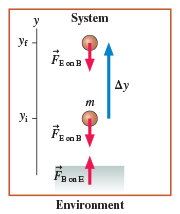
\includegraphics[width=0.4\textwidth]{../figures/ball-earth-potential-energy.png}
    \caption{The ball + earth system has gravitation potential energy}%
    \label{fig:ball-earth-model}
\end{figure}

Figure~%
\ref{fig:ball-earth-model} shows a ball of mass
$
    m
$ moving upward from an initial vertical postion
$
    y_\ini
$ to a final vertical position
$
    y_\fin
$%
.

We define our system as the ball earth and their interactions.  Thus,
\begin{equation}
    \Delta E_{\sys} = W_{\ext} = 0
\end{equation}
as the environment does not do work on the system.  The change in the
energy of the system is the sum of the change of kinetic energy and
potential energy over displacement
$
    s
$%
.
\begin{align}
    \Delta E_\sys &= 0 \\
    &= \Delta K_\tot + \Delta U_\mathrm{G}
\end{align}
where
$
    \Delta U_\mathrm{G} = -(W_B + W_E)
$%
.  Since work is the integral of force and displacement,
\begin{equation}
    W_E \approx 0
\end{equation}
Thus,
\begin{align}
    \Delta U_\mathrm{G} &= -W_B \\
    &= \int F_\mathrm{G} \dif s \\
    &= -mg\Delta y
\end{align}
So if the ball changes its vertical position by
$
    \Delta y
$%
, the gravitational potential energy changes by
\begin{equation}
    \Delta U_\mathrm{G} = -W_B = mg\Delta y
\end{equation}

\subsection{Restoring Forces}

\begin{definition}[Restoring Force]
    A force that restores a system an equilibrium position
\end{definition}

An example of a restoring force is when you stretch a rubber band, a
force tries to pull the rubber band back to equilibrium position.

Suppose you have a spring whose \textbf{equilibrium length} is
$
    L_0
$%
, the length of the spring when it is neither pushing nor pulling.  If
you stretch (or compress) the spring, how hard does it push or pull
back?  Experimentally it is found that
\begin{itemize}
    \item
        The force is \emph{opposite the displacement}.  This is what we
        mean by a restoring force.
    \item
        If you don't stretch or compress the spring too much, the force
        is \emph{proportional to the displacement from equilibrium}. The
        farther you push or pull, the larger the force.
\end{itemize}

\begin{figure}
    \centering
    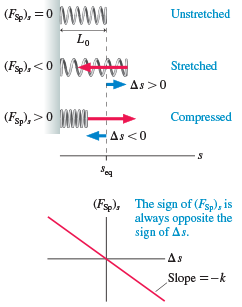
\includegraphics[width=0.6\textwidth]{../figures/spring-properties.png}
    \caption{Spring properties.}%
    \label{fig:spring-properties}
\end{figure}

Figure~%
\ref{fig:spring-properties} shows a spring over a generic
$
    s
$-axis exterting force
$
    \vec{F_\mathrm{Sp}}
$%
.  The graph of the force versus displacement is a straight line with
negative slope, showing that the force is proportional but opposite to
the displacement.  The equation of the straight-line graph passing
through the origin is
\begin{equation}
    (F_\mathrm{Sp})_s = -k\Delta s
\end{equation}
This is known as \textbf{Hooke's law} where
$
    k
$ is the spring constant with units of
$
    \unit{\newton\per\metre}
$%
.  Hooke's laws work for small displacements from equilibrium, but it
will fail if you stretch or compress it too much.

Any string that is hypothetically massless for which Hooke's law is true
at all displacements from equilibrium is an \textbf{ideal spring}.
\begin{Exercise}[title={Pull until it slips}]
    \begin{center}
        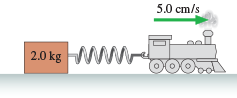
\includegraphics[totalheight=0.2\textheight]{../figures/pull-until-it-slips.png}
        \captionof{figure}{A toy train pulls on the spring until the
        block slips.}%
        \label{fig:pull-until-it-slips}
    \end{center}

    Figure ~%
    \ref{fig:pull-until-it-slips} shows a spring attached to a \SI{2.0}{\kilo\gram}
    block.  The other end of the spring is pulled by a motorized toy
    train that moves forward at \SI{5.0}{\centi\metre\per\second}.  The
    spring constant is \SI{50}{\newton\per\metre}, and the coefficient
    of static friction between the block and the surface is
    $
        0.6
    $%
.    The spring is at equilibrium length at time
    $
        t = \qty{0}{\second}
    $ when the train starts to move When does the block slip?
\end{Exercise}
\begin{Answer}
    \begin{center}
        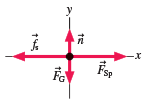
\includegraphics[totalheight=0.2\textheight]{../figures/spring-block-free-body.png}
        \captionof{figure}{The free-body diagram.}%
        \label{fig:spring-block-free-body}
    \end{center}

    Recall that the tension of a massless string pulls equally at \emph{both}
    ends of a string.  This is the same for the spring force:  It pulls
    (or pushes) equally at \emph{both} ends.  As the right end of the
    spring moves, stretching the spring, the spring pulls backward on
    the train \emph{and} forward on the block with equal strength.  As
    the spring stretches, the static friction force on the block
    increases in magnitude to keep the block at rest.

    For the block in static equilibrium
    \begin{equation}
        \sum (\fnet)_x = (\magfsp)_x + (f_s)_x = \magfsp - f_s = 0
    \end{equation}
    where
    $
        \magfsp
    $ is the \emph{magnitude} of the spring force.  By Hooke's law
    $
        \magfsp = k\Delta x
    $%
    , where
    $
        \Delta x = v_x t
    $ is the displacement of the spring from equilibrium.  Thus,
    \begin{equation}
        f_s = \magfsp = k \Delta x
    \end{equation}
    The block slips when the static friction reaches its maximum value
    after the train has moved
    \begin{align}
        \Delta x &= \frac{\sfmax}{k} = \frac{\mu_s mg}{k}\\
        &= \frac{ (0.60)(\qty{2.0}{\kilo\gram})(\qty{9.80}{\metre\per\square\second})
        } {\qty{50}{\newton\per\metre}} \\
        &= \qty{0.235}{\metre}
    \end{align}
    The time at which the block slips is
    \begin{equation}
        t = \frac{\Delta x}{v_x} = \frac{\qty{23.5}{\centi\metre}}{\qty{5.0}
        {\centi\metre\per\second}} = \qty{4.7}{\second}
    \end{equation}
\end{Answer}

\subsubsection{Work Done by Springs}

Hooke's law for a spring is
$
    (F_\mathrm{Sp})_s = -k\Delta s
$%
.  Thus, by the definition of work
\begin{equation}
    W = \int_\ini^\fin (F_\mathrm{Sp})_s \dif s = -(\frac{1}{2}k(\Delta
    s_\fin)^2 - \frac{1}{2}k(\Delta s_\ini)^2)
\end{equation}

\subsection{Elastic Potential Energy}

\begin{figure}
    \centering
    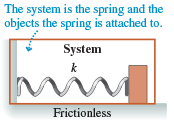
\includegraphics[width=0.4\textwidth]{../figures/block-spring-wall-sys.png}
    \caption{The block + spring + wall system has elastic potential
    energy}%
    \label{fig:block-spring-wall-sys}
\end{figure}

Figure~%
\ref{fig:block-spring-wall-sys} shows a spring exerting a force on a
block while the block moves on a frictionless, horizontal surface.  We
define the system to be the block + spring + wall.

Assuming the spring is massless, it has no kinetic energy.  Instead, the
spring is the interaction between the wall and the block.  Since the
interaction is inside the system, it has an interaction energy, \textbf{the
elastic potential energy}, given by:
\begin{equation}
    \Delta U_\mathrm{sp} = -(W_B + W_W)
\end{equation}
where
$
    W_B
$ is the work the spring does on the block, and
$
    W_W
$%
, is the work the spring does on the wall.  But the wall is rigid and
has no displacement, so
$
    W_W = 0
$ and thus
$
    \Delta U_\mathrm{sp} = -W_B
$%
.  Thus,
\begin{equation}
    U_\mathrm{Sp} = \frac{1}{2}k(\Delta s)^2
\end{equation}

The energy principle for a system with elastic potential energy and no
external interactions is
\begin{equation}
    \Delta E_\sys = \Delta K + \Delta U_\mathrm{Sp} = 0
\end{equation}

\begin{Exercise}[title={An air-track glider compresses a string}]
    In a lab experiment, your instructor challenges you to figure out
    how fast a \SI{500}{\gram} air-track glider is travelling when it
    collides with a horizontal spring attached to the end of the track.
    He pushes the glider and it compresses the string \SI{2.7}{\centi\metre}
    before the glider rebounds.  You then decide to hang the spring on a
    hook and suspend the glider from the bottom end of the spring.  This
    stretches the spring by \SI{3.5}{\centi\metre}.  Based on your
    experiments, how fast was the glider moving?
\end{Exercise}
\begin{Answer}
    Let the system be the wall, the spring, and the glider.  The energy
    principle for our system is
    \begin{align}
        \Delta E_\sys = \Delta K_\tot + \Delta U_\mathrm{Sp} = 0
    \end{align}
    The two free rigid bodys in our system are the wall
    $
        W
    $ and the glider
    $
        G
    $ and will have kinetic energy, thus
    \begin{align}
        \Delta K_\tot = W_W + W_G
    \end{align}
    Since the wall will not move,
    \begin{align}
        \Delta K_\tot &= W_G \\
        &= \frac{1}{2}mv_\fin^2 - \frac{1}{2}mv_\ini^2 \\
        &= \frac{1}{2}0^2 - \frac{1}{2}mv_\ini^2 \\
        &= -\frac{1}{2}mv_\ini^2
    \end{align}
    By the definiiton of elastic potential energy:
    \begin{align}
        \Delta U_\mathrm{Sp} &= \frac{1}{2}k(\Delta x_\fin)^2 - \frac{1}
        {2}k(\Delta x_\ini)^2 \\
        &= \frac{1}{2}k(\Delta x_\fin)^2 - \frac{1} {2}k(0)^2 \\
        &= \frac{1}{2}k(\Delta x_\fin)^2
    \end{align}
    Going back to the energy principle of our system we get,
    \begin{equation}
        \Delta E_\sys = -\frac{1}{2}mv_\ini^2 + \frac{1}{2}k(\Delta x_\fin)^2
        = 0
    \end{equation}
    Solving for
    $
        v_\ini
    $%
    ,
    \begin{align}
        -\frac{1}{2}mv_\ini^2 + \frac{1}{2}k(\Delta x_\fin)^2 &= 0 \\
        -\frac{1}{2}mv_\ini^2 &= -\frac{1}{2}k(\Delta x_\fin)^2 \\
        mv_\ini^2 &= k(\Delta x_\fin)^2 \\
        v_\ini &= \sqrt{\frac{k(\Delta x_\fin)^2}{m}} = \sqrt{\frac{k}{m}}
        \Delta x_\fin
    \end{align}
    You realize you need to find the spring constant
    $
        k
    $%
.    To do so you suspended your glider from the spring vertically, and
    the glider was in equilibrium and not moving.  Thus,
    \begin{equation}
        \fnet = 0
    \end{equation}
    Thus, the force of gravity is the same as the force of the spring on
    the glider.  From Hooke's law,
    \begin{equation}
        \magfsp = k|\Delta y| = mg
    \end{equation}
    We solve for
    $
        k
    $
    \begin{equation}
        k=\frac{mg}{\Delta y}
    \end{equation}
    Now we can solve for
    $
        v_\ini
    $
    \begin{equation}
        v_\ini = \sqrt{\frac{\frac{mg}{\Delta y}}{m}} \Delta x_\fin
    \end{equation}

\end{Answer}

\subsection{Elastic Collisions}

\begin{definition}[Perfectly Elastic Collision]
    A collision in which mechanical energy is conserved.
\end{definition}

\begin{figure}
    \centering
    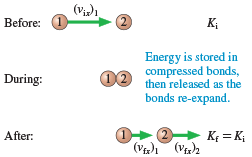
\includegraphics[width=0.4\textwidth]{../figures/perfectly-elastic-collision.png}
    \caption{A perfectly elastic collision.}%
    \label{fig:perfectly-elastic-collision}
\end{figure}

Figure~%
\ref{fig:perfectly-elastic-collision} shows a perfectly elastic
collision of a ball of mass
$
    m_1
$ having initial velocity
$
    (v_{\ini x})_1
$%
, with a ball of mass
$
    m_2
$ thats initially at rest.  The balls velocities after the collision are
$
    (v_{\fin x})_1
$ and
$
    (v_{\fin x})_2
$%
.  This collision \textbf{must objey the conservation of momentum law
and conservation of mechanical energy}.

The conservation of momentum law is not enough as there are two unknowns
of final velocities:
\begin{equation}
    m_1(v_{\ini x})_1 + m_2(v_{\ini x})_2 = m_1(v_{\fin x})_1 + m_2(v_{\fin
    x})_2
\end{equation}

The mechanical energy before and after the collision is purely kinetic
energy.  Thus,
\begin{equation}
    \Delta K_\tot = \Delta( \frac{1}{2}m_1(v_x)_1^2 ) + \Delta( \frac{1}
    {2}m_2(v_x)_2^2 ) = 0
\end{equation}

\subsection{Conservative and Nonconservative Forces}

A system in which particles interact gravitationally or elastically has
a potential energy.  But do all forces have potential energies?  Is
there a ``tension potential energy'' or a ``friction potential energy''?
If not, what's special about the gravitational and elastic forces?  What
conditions must an interaction satisfy to have an assosciated potential
energy?

\begin{figure}
    \centering
    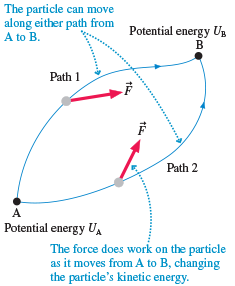
\includegraphics[width=0.4\textwidth]{../figures/two-possible-paths.png}
    \caption{A particle can move from A to B along either of two paths.}
    \label{fig:two-possible-paths}
\end{figure}

Figure~%
\ref{fig:two-possible-paths} shows a particle that can move from point A
to point B along two possible paths while a force
$
    \vec{F}
$ acts on it.  The force experienced in path 1 is not the same as the
force experienced along path 2.  The force change's the particles speed,
so the particle's kinetic energy when it arrives at B differes from the
kinetic it had when it left A.

Assuming there is kinetic energy
$
    U
$ assosciated with force
$
    \vec{F}
$%
.  What restrictions does this place on
$
    \vec{F}
$%
?  There are three steps in the logic:
\begin{enumerate}
    \item
        Potential energy is the energy of position.
        $
            U
        $ depends only where the particle is, not how it got there.  The
        system has one value of potential energy wehn the particle is at
        A, a different value when the particle is at B. Thus, the change
        in potential energy,
        $
            \Delta U = U_\mathrm{B} - U_\mathrm{A}
        $%
        , is the same whether the particle moves along path 1, or path
        2.
    \item
        Potential energy is transformed into kinetic energy, with
        $
            \Delta K = - \Delta U
        $%
.        If
        $
            \Delta U
        $ is independent of the path followed, then
        $
            \Delta K
        $ is also independent of the path.  Thus, the particle has the
        same kinetic energy at B no matter which path it follows.
    \item
        According to the energy principle, the change in the particle's
        kinetic energy is equal to the work done on the particle by the
        force
        $
            \vec{F}
        $%
.        That is,
        $
            \Delta K = W
        $%
.        Because the
        $
            \Delta K
        $ is independent of the path followed, it \emph{must} be the
        case that \textbf{the work done by the force
        $
            \vec{F}
        $ as the particle moves from A to B is independent of the path
        followed}
\end{enumerate}
A force for which the work done on a particle as it moves from an
initial to a final position is independent of the path followed is
called a \textbf{conservative force}.  A potential energy can be
assosciated with any conservative force.  The potential-energy
difference between an initial position i and a final position f is
\begin{equation}
    \Delta U = -W_\mathrm{c} \left(\ini\to\fin\right)
\end{equation}
where the notation
$
    W_\mathrm{c} \left(\ini\to\fin\right)
$ is the work done by a conservative force as the particle moves along
\emph{any} path from i to f.  The most important implication of this is
that when a system changes from i to f, the change in potential energy
only depends on i and f.  It does not depend on how it got from i to f.

A force is called \emph{conservative} because it does not contribute to
any loss of mechanical energy.  Forces like friction might turn kinetic
energy into heat, so they aren't conservative.

\subsection{Force and Potential Energy}

Since we can find the energy of an interaction--potential energy--by
calculating the work the interaction force does inside the system, we
can reverse this and find the force knowing the work.

The force is the negative of the derivative of potential energy with
respect to position.
\begin{equation}
    F_s = -\od{U}{s}
\end{equation}
\begin{proof}
    We defined the change in potential energy to be
    $
        \Delta U = W_\mrint
    $%
.    Suppose an object undergoes a very small displacement
    $
        \Delta s
    $%
    , so small the interaction force
    $
        \vec{F}
    $ is essentially constant.  The work does by a constant force is
    $
        W=F_s \Delta s
    $%
    , where
    $
        F_s
    $ is the component of
    $
        \vec{F}
    $ parallel to the displacement.  During this small displacement, the
    system's potential energy changes by
    \begin{equation}
        \Delta U = -W_\mrint = -F_s \Delta s
    \end{equation}
    We solve for
    $
        F_s
    $
    \begin{equation}
        F_s = -\frac{\Delta U}{\Delta s}
    \end{equation}
    Since we defined this as a \emph{very small} change in
    $
        s
    $%
    :
    \begin{equation}
        F_s = \lim_{\Delta s\to0} \left(-\frac{\Delta U}{\Delta s}\right)
        = -\od {U}{s}
    \end{equation}
\end{proof}
As an example, consider the elastic potential energy
$
    U_\mathrm{Sp} = \frac{1}{2}kx^2
$ for a horizontal spring where
$
    x_\mathrm{eq} = 0
$ so that
$
    \Delta x = x
$%
.  If an object attached to the spring at position
$
    x
$%
, the force on the object is
\begin{equation}
    F_x = -\od{U_\mathrm{Sp}}{x} = \od{}{x}\left(\frac{1}{2}kx^2\right)
    = -kx
\end{equation}

\subsection{Dissipative Forces and Thermal Energy}

\subsubsection{Energy at the Microscopic Level}

\begin{figure}
    \centering
    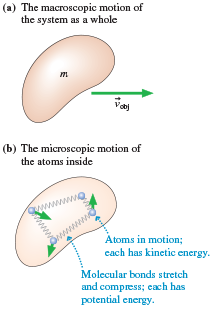
\includegraphics[width=0.4\textwidth]{../figures/micro-vs-macro.png}
    \caption{Two perspectives of motion and energy.}
    \label{fig:micro-vs-macro}
\end{figure}

Figure~\ref{fig:micro-vs-macro} shows two different perspectives on the same object.
In the macrophysics perspective of Figure~\ref{fig:micro-vs-macro}a, you can see an object of 
mass $m$ moving as a whole with speed $v_\mathrm{obj}$. As a consequence of it's motion,
the object has macroscopic kinetic energy $K_\mathrm{macro} = \frac{1}{2}mv_\mathrm{obj}^2$.
\begin{remark}
    Micro means small; macro means large. Macrophysics refers to the motion and dynamics
    of an object as a whole; microphysics refers to the motion of atoms within an object.
\end{remark}
Figure~\ref{fig:micro-vs-macro}b is a microphysics view on the same object, where now
we see a system of particles. Each of the atoms jiggling has kinetic energy, and the bonds
between them are like springs and have potential energy.

The kinetic energy of an atom is exceedingly small, but there are enormous numbers of atoms in a 
macroscopic object. We define the total kinetic energy of all atoms, microscopic kinetic energy,
as $K_\mathrm{micro}$ and the total potential energy of all the bonds, microscopic potential energy,
as $U_\mathrm{micro}$.

The combined microscopic kinetic and potential energy of the atoms--the energy of jiggling atoms and
stretching bonds--is called the \textbf{thermal energy} of the system:
\begin{equation}
    E_\mathrm{th} = K_\mathrm{micro} + U_\mathrm{micro}
\end{equation}

\subsubsection{Dissipative Forces}

Forces such as friction and drag causes the macroscopic kinetic energy of a system to be 
\emph{dissipated as thermal energy}. Hence these are called dissipative forces.
For example, Figure~\ref{fig:dissipated-force-example} shows a box being pulled at a constant speed accross a horizontal surface with friction.
The surface and the box are getting warmer but the kinetic energy is not changing. If we define the system to be box + surface, then the increasing thermal energy is entirely due to the 
work being done on the system by the tension in the rope: $\Delta E_\mathrm{th} = W_\mathrm{tension}$.
Since the box is moving with constant velocity, and thus no net force, $T = f_k$. Consequently, the increase in thermal energy due to dissipative force of friction is 
\begin{equation}
    \Delta E_\mathrm{th} = f_k \Delta s
\end{equation}
\begin{remark}
    Dissipative forces always increase the thermal energy; they never decrease it.
\end{remark}
The reason why we didn't simply calculate the work done by friction is that \textbf{the techniques used to calculate the work done on a particle cannot be used to calculate the work done by dissipative forces}.

\begin{figure}
    \centering
    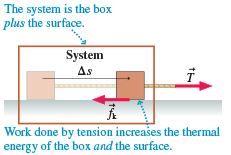
\includegraphics[width=0.4\textwidth]{../figures/dissipated-force-example.png}
    \caption{Work done by tension is dissipated as thermal energy.}
    \label{fig:dissipated-force-example}
\end{figure}

\subsection{Conservation of Energy}

\begin{theorem}[Law of conservation of energy]
    The total energy $E_\sys = E_\mathrm{mech} + E_\th$ of an isolated system is a constant. The kinetic,
    potential, and thermal energy within the system can be transformed into each other, but their sum cannot change. Further,
    the mechanical energy $E_\mathrm{mech} = E + U$ is conserved if the system is both isolated and nondissipative
\end{theorem}

\subsection{The Energy Principle Revisited}

\begin{figure}
    \centering
    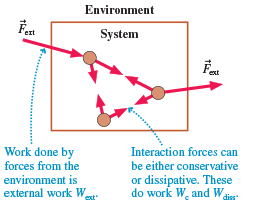
\includegraphics[width=0.4\textwidth]{../figures/both-internal-external-model.png}
    \caption{A system with both internal interactions and external forces.}
    \label{fig:internal-external-model}
\end{figure}
